\chapter{Proof complexity} \label{chap:proof_complexity}

\section{Propositional proof systems}

Proof complexity is the branch of computational complexity and logic that studies the resources that are needed in order to \emph{certify} mathematical statements, rather than of the resources needed to \emph{decide} them. At its core, proof complexity asks if there is a way of writing down proofs of propositional tautologies so that every tautology has short proofs. Such ways of proof writing can be viewed as sets of rules capable of manipulating propositional formulas, deriving new formulas from them. These sets of rules are referred to as \textit{propositional proof systems}. When a formula $\psi$ can be derived from a formula $\varphi$ through the rules of a proof system $Q$, we write $\varphi \stackrel{Q}{\vdash} \psi$ or simply $\varphi \vdash \psi$ when the context is clear. The easiest example of propositional proof system is \textit{Resolution}, based on two single rules:
\[\dfrac{C \lor x \quad D \lor \lnot{x}}{C \lor D} \quad \text{(resolution)} \qquad\qquad \dfrac{C}{C \lor B} \quad \text{(weakening)}\]

For a more detailed discussion on examples of proof systems, see the next section \todo{add ref}. In the seminal paper from which proof complexity originated, defined proof systems as surjective functions $Q : \Sigma^* \to \mathrm{TAUT}$, where the latter is the set of all tautologies, $\mathrm{TAUT} = \{\abk{\varphi} \mid \varphi \text{ a CNF tautology}\}$. The idea behind this definition is that of an algorithm that is able to determine which tautology is proven by a given proof. A modern and more descriptive definition can be achieved through the concept of verifier.

\begin{definition}
    A propositional proof system (p.p.s.) is a verifier $Q$ such that for all formulas $\varphi$ it holds that $\varphi \in \mathrm{TAUT}$ if and only if there is a proof $\pi \in \Sigma^*$ such that $Q(\varphi, \pi) = 1$ and $Q$ runs in time $O((\abs{\varphi} + \abs{\pi})^c)$ for some $c > 0$.
\end{definition}

This if and only if definition can be split in two implications called completeness and soundness. A proof system $Q$ is \textit{complete} if whenever a formula has a $Q$-proof it also is a tautology. Vice versa, $Q$ is \textit{sound} if whenever a formula is a tautology it also has a $Q$-proof. When $\pi$ is a $Q$-proof of $\varphi$, we often write $\pi : Q \vdash \varphi$.

When for each tautology there is a short proof, i.e. $\abs{\pi} = O(\abs{\varphi}^c)$ for some $c > 0$, we say that the proof system is \textit{polynomially bounded}. Proof systems were originally introduced by Cook and Reckhow as a possible way of attacking the $\mathsf{NP}$ vs. $\mathsf{coNP}$ problem. In fact, through the modern definition, its immediate to see that finding a polynomially bounded p.p.s. is equivalent to proving that $\mathsf{NP} = \mathsf{coNP}$.

\begin{proposition}
    There is a polynomially bounded p.p.s. if and only if $\mathsf{NP} = \mathsf{coNP}$ 
\end{proposition}

\begin{proof}

    One can easily prove that $\mathrm{TAUT}$ is $\mathsf{coNP}$-complete. For our purposes, we can omit this proof and assume it to hold. Let $Q$ be a polynomially bounded p.p.s. Then, since for each formula there is a proof of size $\abs{\pi} = O(\abs{\varphi}^c)$ for some $c > 0$, $Q$ is a verifier for $\mathrm{TAUT}$ with polynomial runtime with respect to the input size $\abs{\varphi}$, concluding that $\mathrm{TAUT} \in \mathsf{NP}$. By completeness, we get that $\mathsf{NP} = \mathsf{coNP}$.

    Vice versa, suppose that $\mathsf{NP} = \mathsf{coNP}$. Then, since $\mathrm{TAUT} \in \mathsf{NP}$, there is a polynomial time verifier $V$ for $\mathrm{TAUT}$. In order for it to run in polynomial time, for each formula $\varphi$ there must be at least one witness $t$ such that $\abs{w} = O(\abs{\varphi}^d)$ for some $d > 0$, otherwise reading the witness would always require super-polynomial runtime, raising a contradiction. This concludes that $V$ is a polynomially bounded p.p.s.
\end{proof}

In their programme, Cook and Reckhow outlined a possible roadmap to proving that $\mathsf{NP} \neq \mathsf{coNP}$ through p.p.s. Their idea involved proving that strong proof systems require super-polynomial size proofs for some formulas, to then generalize the various results to any possible proof system, i.e. showing that every proof system has at least one formula that is hard to prove. However, researchers quickly realized that this task would be tedious even for weaker systems. In fact, even after almost 40 years of research in the field, only a few weak systems have been completely outlined (e.g. Resolution). 

The programme has also a second, entirely practical, motivation. Every complete
algorithm that established the satisfiability of a propositional formul, referred to as a \textit{SAT-solver}, implicitly produces a proof of that formula in some proof system. For instance, the DPLL algorithm (Davis-Putnam-Logemann-Loveland) and CDCL solvers (Conflict-driven Clause Learning) produce resolution proofs, while Gr\"obner basis
solvers produce algebraic proofs. A lower bound on proof size in a system
is therefore an unconditional lower bound on the running time of \emph{every}
algorithm of the corresponding kind, regardless of how cleverly it is
implemented. Proof complexity is, from this point of view, the theory of the
limits of automated reasoning.

\section{Common proof systems}

\subsection{Resolution}

The Resolution proof system ($\mathrm{Res}$), introduced by Robinson \todo{add ref}, is the most extensively studied proof system, extensively in automated theorem proving, SAT-solvers and artificial intelligence. Like many weak proof systems, Resolution's proofs are actually \textit{refutations}, i.e. \curlyquotes{proofs} of unsatisfiability of a formula. This is a feature, not an issue: since $\varphi$ is a tautology if and only if $\lnot \varphi$ is unsatisfiable, any refutation of $\lnot \varphi$ is actually a proof of $\varphi$. In many works, the word refutation is often used as a synonym of proof. To help the reader, this won't be the case in this work.

Resolution refutations are based on repeated applications of two simple rules, starting from the axioms of the initial formula:
\[\dfrac{C \lor x \quad D \lor \lnot{x}}{C \lor D} \quad \text{(resolution)} \qquad\qquad \dfrac{C}{C \lor B} \quad \text{(weakening)}\]

Given a CNF formula $\varphi = C_1 \land \ldots \land C_m$, let $\mathrm{Ax}(\varphi) = \{C_1, \ldots, C_m\}$ be the set of axioms of $\varphi$. Then, a Resolution refutation of $\varphi$ is a sequence of clauses $\pi = (D_1, D_2, \ldots, D_t)$ such that for each $i \in [t]$ exactly one of the following holds:
\begin{itemize}
    \item \textit{Axiom}: $D_i \in \mathrm{Ax}(\varphi)$;
    \item \textit{Resolution}: $D_i = \mathrm{Res}(D_j, D_k)$ with $j,k \in [i-1]$;
    \item \textit{Weakening}: $D_i = \mathrm{Weak}(D_j)$ with $j \in [i-1]$.
\end{itemize}

For the last clause $D_t$, it must hold that $D_t = \bot$, where $\bot$ represents the \textit{empty clause}, i.e. the clause that doesn't contain any literal.

\begin{figure}
    \[\begin{array}{rcl}
        D_1 :& \lnot{x_3} & \text{Axiom} \\
        D_2 :& \lnot{x_1} \lor \lnot{x_2} \lor x_3 & \text{Axiom} \\
        D_3 :& x_1 \lor \lnot{x_2} \lor x_3 & \text{Axiom} \\
        D_4 :& \lnot{x_1} \lor \lnot{x_2} & \mathrm{Res}(D_1, D_2) \\
        D_5 :& x_1 \lor \lnot{x_2} & \mathrm{Res}(D_1, D_3) \\
        D_6 :& x_2 \lor x_3 & \text{Axiom} \\
        D_7 :& x_2 \lor \lnot{x_3} & \text{Axiom} \\
        D_8 :& x_2 & \mathrm{Res}(D_6,D_7) \\
        D_9 :& \lnot{x_1} & \mathrm{Res}(D_4, D_8) \\
        D_{10} :& x_1 & \mathrm{Res}(D_5, D_8) \\
        D_{11} :& \bot & \mathrm{Res}(D_9, D_10) \\
    \end{array}\]
    \caption{Example of a Resolution refutation for the formula $(x_2 \lor x_3) \land (x_2 \lor \lnot{x_3}) \land (x_1 \lor \lnot{x_2} \lor x_3) \land (\lnot{x_1} \lor \lnot{x_2} \lor x_3) \land \lnot{x_3}$}
    \label{fig:res_example_1}
\end{figure}

The idea behind the Resolution proof system comes from the propagation of satisfiability underlying the resolution rule and the weakening rule.

\begin{proposition}
    Let $\alpha$ be an assignment. If $\alpha(C \lor x) = 1$ and $\alpha(D \lor \lnot x) = 1$ then $\alpha(C \lor D) = 1$. Similarly, if $\alpha(C) = 1$ then $\alpha(C \lor B) = 1$
\end{proposition}

One can easily prove by induction that if a clause $Z$ is derived through repeated applications of resolution and weakening starting from the axioms then $\alpha(\varphi) = 1$ implies $\alpha(Z) = 1$. When $Z = \bot$, we reach a contradiction since, by definition, the empty clause is unsatisfiable. Therefore, if we're able to derive $\bot$ starting from $\mathrm{Ax}(\varphi)$, we obtain a valid proof of the fact that $\varphi$ must be unsatisfiable. This proves the soundness of Resolution and completeness can be proven in a similar way.

For any fixed natural number $k \in \N$, we define an extension of the Resolution proof system called \textit{Resolution over $k$-DNFs}, denoted $\mathrm{Res}(k)$, first introduced by \todo{add ref}. This proof system works over sets of $k$-DNF formulas, expressed as a disjunction of conjunctions of at most $k$ literals. Its rules are inspired by to those of Resolution, adapting them to manage $k$-DNFs:
\[\begin{array}{rl}
\dfrac{\mathcal{D}_1 \lor \rbk{\bigvee_{j \in J} \ell_j} \quad \mathcal{D}_2 \lor \rbk{\bigwedge_{j \in J} \lnot \ell_j}}{\mathcal{D}_1 \lor \mathcal{D}_2} & \quad \text{(cut)} \\\\

\dfrac{\mathcal{D}_1 \lor \rbk{\bigwedge_{j \in J} \ell_j} \quad \mathcal{D}_2 \lor \rbk{\bigwedge_{j' \in J'} \ell_{j'}}}{\mathcal{D}_1 \lor \mathcal{D}_2 \lor \rbk{\bigvee_{j \in J \cup J'} \ell_j}} &\quad \text{($\land$ introduction)} \\\\

\dfrac{\mathcal{D}_1}{\mathcal{D}_1 \lor \rbk{\bigwedge_{j \in J} \ell_j}} \qquad \dfrac{\mathcal{D} \lor \rbk{\bigwedge_{j \in J \cup J'} \ell_{j}}}{\mathcal{D}_1 \lor \rbk{\bigvee_{j \in J} \ell_j}} &\quad \text{(weakenings)}
\end{array}\]
where $\mathcal{D}_1$ and $\mathcal{D}_2$ are $k$-DNF formulas.

\subsection{Frege systems}

\textit{Frege systems} are a more classical type of propositional proof system, whose proofs are intended to infer tautologies. These proof systems are well known in the classical Logic literature and, furthermore, they work not only with CNF formulas, but also with general Boolean formulas.

Formally, a Frege system is a propositional proof system built from a finite set of axiom schemes and a finite set of rules of inference that can be applied to sets of formulas. An \textit{axiom scheme} is a meta-formula with variables over formulas that can be substituted by any formula. For instance, both $x_1 \land x_2 \to x-1$ and $(x_1 \lor x_2) \land x_2 \to (x_1 \lor x_2)$ are formulas that can be obtained from the axiom schema $(P \land Q) \to Q$, where $P$ and $Q$ are variables over $\mathrm{Fml}(\mathcal{P})$. A \textit{rule scheme} is a typical rule of logical derivation. A prominent example of a schema rule is the \textit{Modus Ponens} (MP), defined as:
\[\dfrac{P \qquad P \to Q}{Q}\]

Modus Ponens allows to cut implications from formulas of the form $P \to Q$ once the formula $P$ alone is derived. We can define different Frege systems introducing different axiom schemes. Nonetheless, Reckhow proved that all Frege systems are polynomially equivalent to each other \todo{add ref}, meaning that the axiom scheme and rule scheme chosen is not relevant, up to some polynomial factor (see Section \todo{add ref} for an explanation of polynomial equivalence). Therefore, we don't actually care about which rules and axioms are used in our Frege system. This allows us to restrict our interest to a standardized Frege system, known in the literature as \textit{Hilbert's propositional proof system}, denoted with $\mathrm{F}$ or $\mathrm{Frege}$. The rule scheme of this proof system allows only the use of Modus Ponens over the following standard axiom scheme $\mathrm{Ax}(\mathrm{F})$ of Hilbert-style systems for propositional logic:

\[\begin{array}{rll}
    (1) \quad & A \to B \to (A \land B) \\
    (2) \quad & (A \land B) \to A & \land \text{ rules} \\
    (3) \quad & (A \land B) \to B \\[1em]
    (4) \quad & A \to (A \lor B) \\
    (5) \quad & B \to (A \lor B) & \lor \text{ rules} \\
    (6) \quad & (A \to C) \to (B \to C) \to ((A \lor B) \to C) \\[1em]
    (7) \quad & (\bot \to A) \\
    (8) \quad & (A \to \bot) \to \neg A & \neg \text{ rules} \\
    (9) \quad & A \to (\neg A \to \bot) \\
    (10) \quad & (\neg A \to \bot) \to A \\[1em]
    (11) \quad & A \to A \\
    (12) \quad & A \to (B \to A) & \to \text{ rules} \\
    (13) \quad & (A \to (B \to C)) \to ((A \to B) \to (A \to C))
\end{array}\]

Given a formula $A$, an F-proof of $A$ is sequence of formulas $\pi = (A_1, \ldots , A_t)$ such that each $i \in [t]$ exactly one of the following holds:
\begin{itemize}
    \item \textit{Axiom}: $A_i \in \mathrm{Ax}(\mathrm{F})$;
    \item \textit{Modus Ponens}: $A_i = \mathrm{MP}(A_j, A_k)$ with $j,k \in [i-1]$.
\end{itemize}

For the last formula $A_t$, it must hold that $A = A_t$. The soundness of F comes immediately from the soundness of Modus Ponens, something that assumed as an axiom in standard settings of classical Logic. Completeness follows similarly.

\textit{Extended Frege systems}, denoted with $\mathrm{EF}$, are Frege systems augmented with an \textit{extension rule} that allows the introduction of new variables that abbreviate more complex formulas.
\begin{itemize}
    \item \textit{Extension}: $A_i = q \leftrightarrow B$ where $q$ is a new variable that never appeared before and $B$ is any propositional formula.
\end{itemize}

Intuitively, this rule allows us to write shorter proofs by encoding partial statements are single variables and use it in the proof, instead of carrying over the initial statement across the whole proof. In some sense, Frege proofs can be viewed as proofs that reason about polynomial size Boolean
formulas, while Extended Frege proofs as proofs that reason about polynomial size Boolean circuits.

\subsection{Algebraic systems}

\textit{Algebraic proof systems} are proof systems based on polynomials. 
These systems can be used to witness the fact that a system of polynomial equations over a the polynomial ring $\F[x_1, \ldots, x_n]$ is unsolvable; equivalently, that the polynomials do not have a common root.

Consider a CNF formula $\varphi$ defined over $x_1, \ldots, x_n$. The formula can be easily encoded as a set of polynomials such that the formulas is unsatisfiable if and only if such set of polynomials has no solution. We map each clause of $\varphi$ to an equation in the following way:
\[\bigvee_{i \in I} x_i \lor \bigvee_{j \in J} \lnot x_j \mapsto \prod_{i \in I} x_i \prod_{j \in J} (1-x_j) = 0\] 

where $I$ and $J$ are, respectively, the set of positive and negative literals of the clause. For each clause $C$, its corresponding polynomial is denoted with $P(C)$. The formula $\varphi$ is unsatisfiable if and only if the system $\Phi = \{P(C)\}_{C \in \varphi} \cup \{x_i^2 - x_i = 0\}_{i \in [n]}$ has no solutions. In particular, the latter set of equations is used to restrict all possible solutions to those that give Boolean values to $x_1, \ldots, x_n$.

After this transformation is made, the question of whether a formula is unsatisfiable is reduced to the question of a set of polynomial equations is unsolvable. Algebraic tools can then be used in order to decide unsatisfiability of the original formulas. We notice that, under this framework, truth is inversely represented: the value $0$ represents truth, while $1$ represents falsity.

Two particular algebraic proof systems are extensively studied in proof complexity: Nullstellensatz and Polynomial Calculus. \textit{Nullstellensatz} (NS) is a static algebraic proof system, i.e. one that doesn't use rules of inference, based on Hilbert's Nullstellensatz, which states that given $m$ polynomials $p_1, \ldots, p_m$ the system $p_1(x) = p_2(x) = \ldots = p_m(x) = 0$ is unsolvable if and only if 1 lies in their generated ideal, i.e. there are $m$ polynomials $g_1, \ldots , g_m$ such that $\sum_{j = 1}^m g_jp_j = 1$. For any CNF $\varphi$, an NS-proof of $\varphi$ is the set of polynomials $\pi = \{g_1, \ldots, g_m, h_1, \ldots, h_m\}$ such that:
\[\sum_{j = 1}^m g_jp_j + \sum_{i = 1}^n h_i(x_i^2-x_i) = 1\]
where $p_j = P(C_j)$ for each $j \in [m]$.

\textit{Polynomial Calculus} (PC) is a dynamic proof system based on two rules:
\[\dfrac{p \qquad q}{\alpha p+ \beta q} \quad \text{(linear combination)} \qquad\qquad \dfrac{p}{xp} \quad \text{(multiplication)}\]
where $\alpha,\beta \in \F$ and $x \in \{x_1, \ldots, x_n\}$. A PC-proof of the CNF $\varphi$ is a sequence of polynomials $\pi = (f_1, \ldots, f_t)$ such that each $i \in [t-1]$ exactly one of the following holds:
\begin{itemize}
    \item \textit{Axiom}: $f_i$ is the polynomial of some equation in $\Phi$
    \item \textit{Linear combination}: $f_i = \mathrm{Sum}(f_j, f_k)$ with $j,k \in [i-1]$
    \item \textit{Multiplication}: $f_i = \mathrm{Mul}(f_j)$ with $j \in [i-1]$
\end{itemize}

For the last polynomial $f_t$, it must hold that $f_t = 1$. The soundness of PC can be proven in way similar to Resolution: if we assume that the system of equations $\Pi$ has a solution, the equality with 0 can be propagated down to the last polynomial $f_t = 1$, raising a contradiction. Completeness follows similarly.

\subsection{Optimization-based systems}

\textit{Optimization-based proof systems} are proof systems based on linear programming. All such proof systems are variants of the \textit{Cutting Planes} (CP) proof system, a refutational method derived from 0-1 integer programming. In CP, any CNF formula $\varphi$ is converted into an equivalent system of linear inequalities (similar to how algebraic systems convert them into equations) whose integer binary solutions correspond directly to the satisfying assignments of $\varphi$. Each clause of a formula $\varphi$ is mapped to an inequality in the following way:
\[\bigvee_{i \in I} x_i \lor \bigvee_{j \in J} \lnot x_j \mapsto \sum_{i \in I} x_i + \sum_{j \in J} (1-x_j) \geq 1\] 

For each clause $C$, its corresponding inequality is denoted with $E(C)$. Interpreting truthness as 1 and falseness as 0, the formula $\varphi$ is unsatisfiable if and only if the system $\Phi  = \{E(C)\}_{C \in \varphi} \cup \{x_i \geq 0; x_i \leq 1\}_{i \in [n]}$ has no an integer solution. The set of all feasible solutions for this system yield a polytope $P$. While any Boolean point in $P$ yields a satisfying assignment for $F$, an unsatisfiable formula $F$ may still leave non-integer (fractional) points within $P$. CP eliminates these fractional solutions using the \textit{Chvátal-Gomory cut rule}. In particular, CP is based on the two following rules:
\[\dfrac{\sum_{i \in [n]} \alpha_i x_i \geq \gamma \qquad \sum_{i \in [n]} \beta_{i} x_{i} \geq \delta}{\sum_{i \in [n]} (\alpha_i + \beta_i) x_i \geq \gamma + \delta} \quad \text{(linear combination)}\]
\[\dfrac{\sum_{i \in [n]}  \eta\alpha_i x_i \geq \gamma}{\sum_{i \in [n]} \alpha_ix_i \geq \floor{\frac{\gamma}{\eta}}} \quad \text{(cut)}\]

Formally, a CP-proof of the CNF $\varphi$ is a sequence of inequalities $\pi = (f_1, \ldots, f_t)$ such that each $i \in [t-1]$ exactly one of the following holds:
\begin{itemize}
    \item \textit{Axiom}: $f_i \in \Phi$
    \item \textit{Linear combination}: $f_i = \mathrm{Sum}(f_j, f_k)$ with $j,k \in [i-1]$
    \item \textit{Multiplication}: $f_i = \mathrm{Cut}(f_j)$ with $j \in [i-1]$
\end{itemize}

For the last inequality $f_t$, it must hold that $f_t : 0 \geq 1$ to ensure a contradiction.

\subsection{Tree-like systems}

Consider again the refutation in \Cref{fig:res_example_1}. To make things easier to read, we can represent this refutation as a Directed Acyclic Graph (DAG) by connecting clauses with lines. These refutations are called \textit{DAG-like refutations}.

\begin{figure}[H]
    \centering
    \resizebox{0.8\hsize}{!}{
        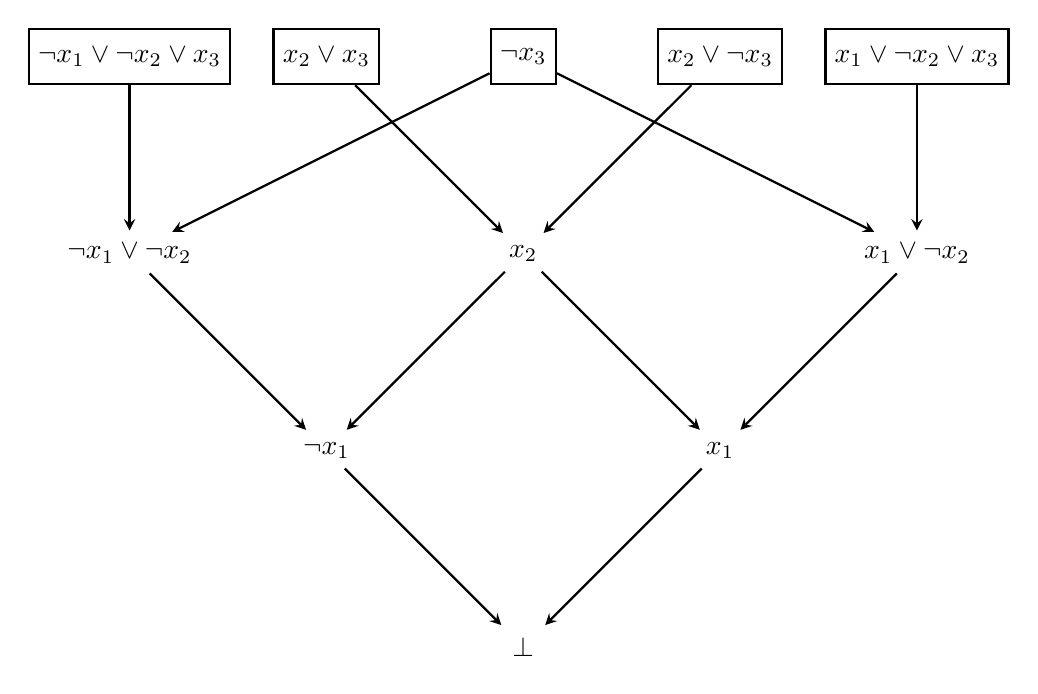
\begin{tikzpicture}[->,>=stealth,shorten >=1pt,auto,node distance=2.5cm, thick,main node/.style={scale=0.9,circle,draw,font=\sffamily\normalsize}]
            \node [rectangle, draw, minimum height=20](1) []{$\lnot{x_1} \lor \lnot{x_2} \lor x_3$};
            \node [rectangle, draw, minimum height=20](2) [right of=1]{$x_2 \lor x_3$};
            \node [rectangle, draw, minimum height=20](3) [right of=2]{$\lnot{x_3}$};
            \node [rectangle, draw, minimum height=20](4) [right of=3]{$x_2 \lor \lnot{x_3}$};
            \node [rectangle, draw, minimum height=20](5) [right of=4]{$x_1 \lor \lnot{x_2} \lor x_3$};

            \node (6) [below of=1]{$\lnot{x_1} \lor \lnot{x_2}$};
            \node (x) [below of=2]{};
            \node (7) [below of=3]{$x_2$};
            \node (y) [below of=4]{};
            \node (8) [below of=5]{$x_1 \lor \lnot{x_2}$};

            \node (9) [below of=x]{$\lnot{x_1}$};
            \node (10) [below of=y]{$x_1$};
            \node (z) [below of=7]{};
            
            \node (11) [below of=z]{$\bot$};
        
            \path[every node/.style={font=\sffamily\small}]
                (1) edge (6)
                (2) edge (7)
                (3) edge (6)
                (3) edge (8)
                (4) edge (7)
                (5) edge (8)

                (6) edge (9)
                (7) edge (9)
                (7) edge (10)
                (8) edge (10)

                (9) edge (11)
                (10) edge (11)
                ;
        \end{tikzpicture}
    }
    \caption{DAG-like representation of the refutation in \Cref{fig:res_example_1}.}
    \label{fig:dag_res_proof}
\end{figure}

We observe that the definition of Resolution refutation allows rules to be applied more than once onto each clause of the proof. There may also be multiple copies of a single clause, each obtained by applying different rules.
When each copy of a clause is used only once as premise in the whole proof, we say that the refutation is \textit{tree-like} (named after the fact that the graph becomes a tree). This restriction implies that if we want to use a clause multiple times then it must be derived again, usually starting from the same axioms.

\begin{figure}[H]
    \centering
    
    \resizebox{1\hsize}{!}{
        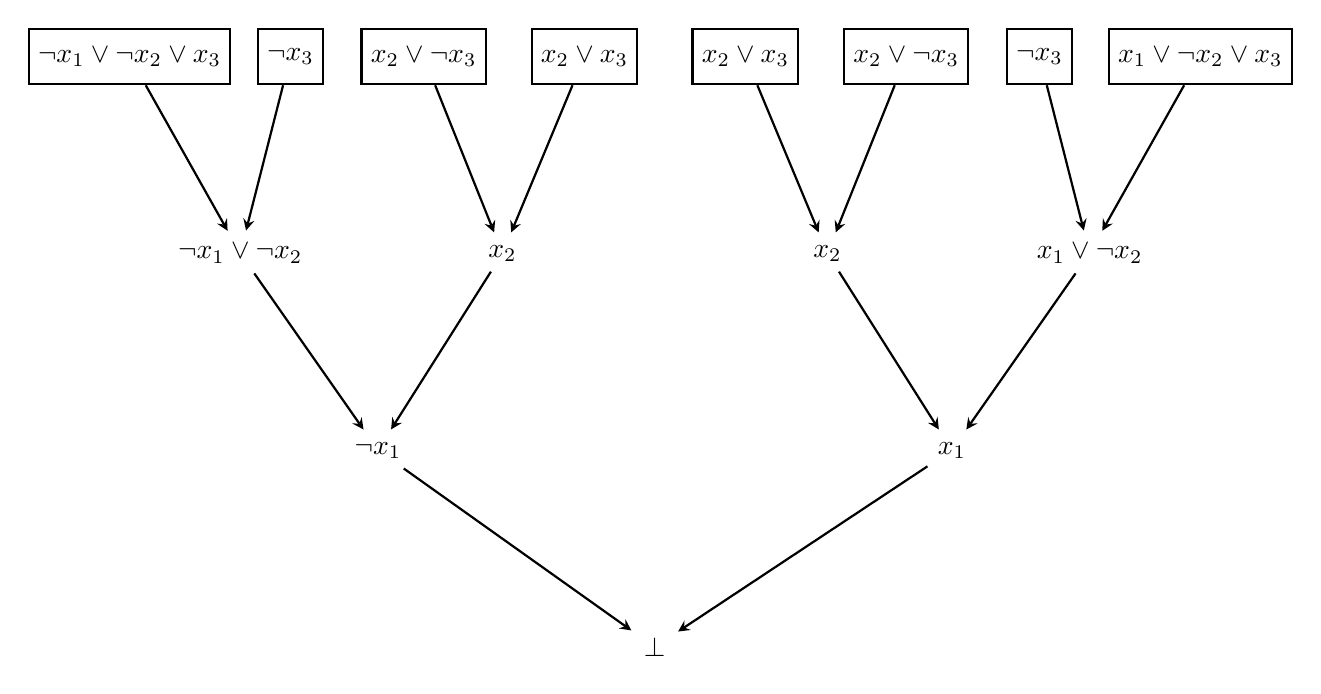
\begin{tikzpicture}[->,>=stealth,shorten >=1pt,auto,node distance=2.5cm, thick,main node/.style={scale=0.9,circle,draw,font=\sffamily\normalsize}]
            \node [rectangle, draw, minimum height=20](1) []{$\lnot{x_1} \lor \lnot{x_2} \lor x_3$};
            \node [rectangle, draw, minimum height=20](2) [right of=1, xshift=-13]{$\lnot{x_3}$};
            \node [rectangle, draw, minimum height=20](3) [right of=2, xshift=-23]{$x_2 \lor \lnot{x_3}$};
            \node [rectangle, draw, minimum height=20](4) [right of=3, xshift=-13]{$x_2 \lor x_3$};
            \node [rectangle, draw, minimum height=20](5) [right of=4, xshift=-13]{$x_2 \lor x_3$};
            \node [rectangle, draw, minimum height=20](6) [right of=5, xshift=-13]{$x_2 \lor \lnot{x_3}$};
            \node [rectangle, draw, minimum height=20](7) [right of=6, xshift=-23]{$\lnot{x_3}$};
            \node [rectangle, draw, minimum height=20](8) [right of=7, xshift=-13]{$x_1 \lor \lnot{x_2} \lor x_3$}; 

            \node (9)[below of=1, xshift=40]{$\lnot{x_1} \lor \lnot{x_2}$};
            \node (10)[below of=3, xshift=28.5]{$x_2$};
            \node (11)[below of=6, xshift=-28.5]{$x_2$};
            \node (12)[below of=8, xshift=-40]{$x_1 \lor \lnot{x_2}$};

            \node (13)[below of=10, xshift=-45]{$\lnot{x_1}$};
            \node (14)[below of=11, xshift=45]{$x_1$};

            \node (15)[below of=13, xshift=100]{$\bot$};
        
            \path[every node/.style={font=\sffamily\small}]
                (1) edge (9)
                (2) edge (9)
                (3) edge (10)
                (4) edge (10)
                (5) edge (11)
                (6) edge (11)
                (7) edge (12)
                (8) edge (12)

                (9) edge (13)
                (10) edge (13)
                (11) edge (14)
                (12) edge (14)

                (13) edge (15)
                (14) edge (15)
                ;
        \end{tikzpicture}
    }
    
    \caption{Tree-like adaptation of the refutation in \Cref{fig:res_example_1}.}
    \label{fig:treelike_res_proof}
\end{figure}

This sub-system of Resolution is called \textit{tree-like Resolution}, denoted with $\mathrm{Res}^*$. The same idea can also be applied to other dynamic systems, obtaining sub-systems like $\mathrm{Res}^*(k), \mathrm{F}^*$ and $\mathrm{PC}^*$. Generally, tree-like sub-system require longer proofs due to the impossibility of reusing derived clauses.

\section{Simulations between proof systems}

To compare the relative strength of different propositional proof systems, we introduce the notion of efficient simulation. This notion comes in a natural way by adapting the idea of polynomial time reduction.

\begin{definition}
    Given two proof systems $P,Q$, we say that $Q$ polynomially simulates $P$, written $P \leq_p Q$ if there is a polynomial time computable function $f : \Sigma^* \to \Sigma^*$ such that for all tautologies $\varphi$ if $\pi$ is a $P$-proof of $\varphi$ then $f(\pi)$ is a $Q$-proof of $\varphi$.
\end{definition}

Intuitively, this means that there is an efficient algorithms transforming $P$-proofs into $Q$-proofs for the same formula. Consider the binary relation $\leq_p$. Similarly to reductions, this formula forms a partial order. In particular, for any pair $P,Q$ of proof systems we say that:
\begin{itemize}
    \item $P$ and $Q$ are \textit{polynomially equivalent} when $P \leq_p Q$ and $Q \leq_p P$. We often write $P \equiv_p Q$ when this holds.
    \item $P$ is \textit{superpolynomially weaker} than $Q$ when $P \leq_p Q$ but $Q \not\leq_p P$
    \item $P$ and $Q$ are \textit{incomparable} when $P \not\leq_p Q$ and $Q \not\leq_p P$
\end{itemize}

It's easy to see that for any dynamic proof system $Q$ it holds that $Q^* \leq_p Q$ since any $Q^*$-proof is also a $Q$-proof. Vice versa, however, it commonly holds that $Q \not\leq_p Q^*$, making tree-like systems typically weaker than their DAG-like counterpart. For instance, standard techniques can prove that the Ordering Principle formula $\mathrm{OP}_n$ is an hard formula for tree-like Resolution but an easy one for Resolution, implying that $\mathrm{Res} \not\leq_p \mathrm{Res}^*$.

When it comes to comparing Resolution with Nullstellensatz and Polynomial Calculus, they're both incomparable with it. This is due to the fact that negative literals easily blow up the size of the proof due to the increase in the number of monomials when expanded. To fix this, we can consider a variant of Polynomial Calculus referred to as \textit{Polynomial Calculus with Resolution} (PCR) -- a name that pretty much says it all -- where for each variable $x_i$ we add a new variable $\overline{x_i}$ in order to map negative literals $\lnot x_i$ directly to this new variable.
\[\bigvee_{i \in I} x_i \lor \bigvee_{j \in J} \lnot x_j \mapsto \prod_{i \in I} x_i \prod_{j \in J} \overline{x_j} = 0\]

All the other standard simulations and separations between proof systems are omitted and summarized in \Cref{fig:simulations}.

\begin{figure}[H]
    \centering
    \resizebox{0.5\textwidth}{!}{
        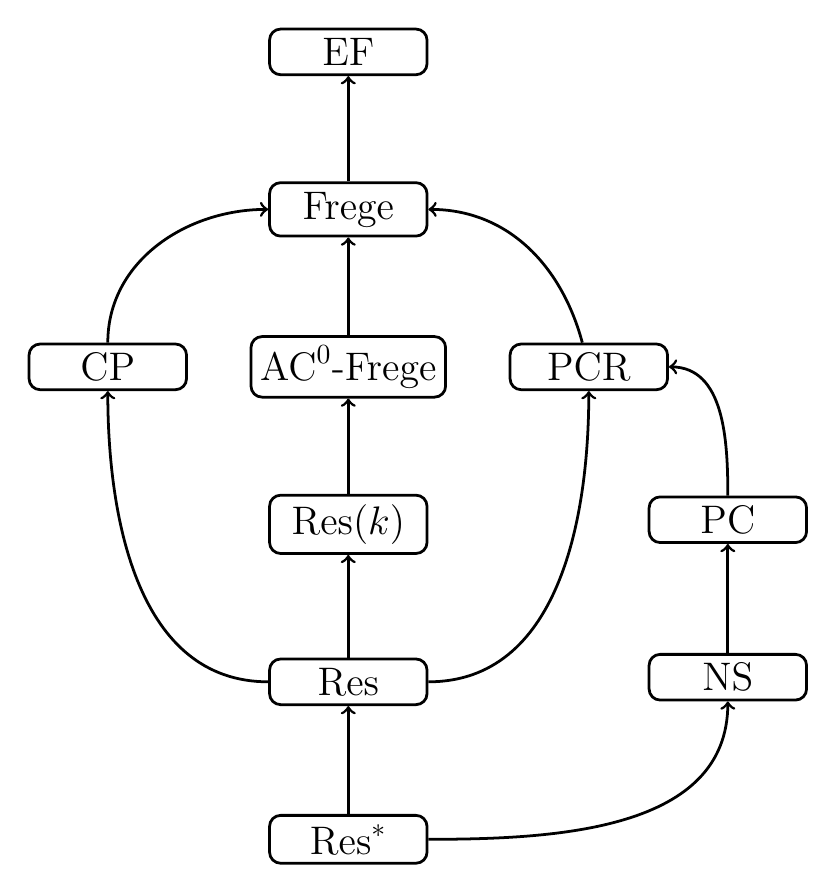
\begin{tikzpicture}[node distance=2cm and 1.8cm, font=\Large, line width=1pt ]
            % --- Nodes Placement ---
            \node[rectangle, rounded corners, draw, minimum width = 2cm] (EF) {$\mathrm{EF}$};
            \node[rectangle, rounded corners, draw, minimum width = 2cm] (F) [below of = EF] {$\mathrm{Frege}$};
            \node[rectangle, rounded corners, draw, minimum width = 2cm] (AC0F) [below of = F] {$\mathrm{AC}^0$-$\mathrm{Frege}$};
            \node[rectangle, rounded corners, draw, minimum width = 2cm] (ResK) [below of = AC0F] {$\mathrm{Res}(k)$};
            \node[rectangle, rounded corners, draw, minimum width = 2cm] (Res) [below of = ResK] {$\mathrm{Res}$};
            
            \node[rectangle, rounded corners, draw, minimum width = 2cm] (CP) [left of = AC0F, xshift = -30] {$\mathrm{CP}$};
            \node[rectangle, rounded corners, draw, minimum width = 2cm] (PCR) [right of = AC0F, xshift = 30] {$\mathrm{PCR}$};
            \node[rectangle, rounded corners, draw, minimum width = 2cm] (PC) [below right of = PCR, xshift=10, yshift=-15] {$\mathrm{PC}$};
            \node[rectangle, rounded corners, draw, minimum width = 2cm] (NS) [below of = PC] {$\mathrm{NS}$};
            \node[rectangle, rounded corners, draw, minimum width = 2cm] (ResStar) [below of = Res] {$\mathrm{Res}^*$};

            % --- Direct Straight Connections ---
            \draw[->] (Res) -- (ResK);
            \draw[->] (ResK) -- (AC0F);
            \draw[->] (AC0F) -- (F);
            \draw[->] (F) -- (EF);
            
            \draw[->] (ResStar) -- (Res);
            \draw[->] (NS) -- (PC);
            
            % --- Curved Connections ---
            \draw[->] (ResStar) to[out=0, in=270] (NS);
            \draw[->] (Res) to[out=180, in=270] (CP);
            \draw[->] (Res) to[out=0, in=270] (PCR);

            \draw[->] (PC) to[out=90, in=0] (PCR);
            \draw[->] (CP) to[out=90, in=180] (F);
            \draw[->] (PCR) to[out=105, in=0] (F);
        \end{tikzpicture}
    }
    
    \caption{Simulations between standard proof systems.}
    \label{fig:simulations}
\end{figure}
\todo{add references for simulations (also inside the image)}

\section{Complexity measures for proof systems}

Complexity measures lie at the heart of proof complexity. These measures provide a rigorous language to measure if a minimal proof must be short or long, allowing us to evaluate how different systems perform on proving a common statement. Different measures highlight different facets of a proof, often interlinking them. By analyzing these measures, we gain a deeper understanding of the inherent difficulty of logical reasoning, even from an algorithmic prospective.

Resolution is the quintessential proof system when it comes to complexity measures. Consider a Res-proof $\pi$. For any clause $C$, let $\abs{C}$ denote the number of literals in $C$. Our main complexity measure of interest is The \textit{size} of $\pi$, written as $\abs{\pi}$, corresponding to the total number of literals inside it, i.e. $\abs{\pi} = \sum_{D_i \in \pi} \abs{D_i}$. For instance, the refutation in \Cref{fig:res_example_1} has size $19$. In a natural way, the size of the proof corresponds to the number of symbols used to describe the witness of the verifier-based definition of the proof system. For any formula $\varphi$ with $m$ clauses over $n$ variables, the Resolution size of $\varphi$, written as $\mathrm{size}_{\mathrm{Res}}(\varphi)$, is the minimum size across all Res-proofs of $\varphi$ (equivalently, across all refutations of $\lnot \varphi$).
\[\mathrm{size}_{\mathrm{Res}}(\varphi) = \min_{\pi : \mathrm{Res} \vdash \varphi} \abs{\pi}\]

Finding the Resolution size of a formula tells us the exact minimum number of symbols in a witnessing string for the given formula. Proving the existence of at least one formula $\varphi$, with $m$ clauses over $n$ variables, whose Resolution size is super-polynomial with respect to $\abs{\varphi} = \Theta(n+m)$ is sufficient to conclude Resolution is not polynomially bounded. Haken \todo{add ref} was the first to show that one such formula is the Pigeonhole Principle formula $\mathrm{PHP}^{n+1}_{n}$, which has size $2^{\Theta(n)}$. This result not only implies that Resolution is polynomially bounded, but it also implies that every CNF formula that implicitly describes the Pigeonhole Principle is hard for Resolution. Since this combinatorial principle is at the foundation of mathematics, this makes Resolution weak against a wide subset of formulas. 

A natural complexity measure related with size is the \textit{length} of a proof, which measures the total number of clauses inside $\pi$, i.e. the number of steps in the proof. The Resolution length of a formula $\varphi$, written as $\mathrm{length}_{\mathrm{Res}}(\varphi)$, is the minimum length across all Res-proofs of $\varphi$. One can easily prove that $\mathrm{length}_{\mathrm{Res}}(\varphi) \leq \mathrm{size}_{\mathrm{Res}}(\varphi) \leq n \cdot \mathrm{length}_{\mathrm{Res}}(\varphi)$ holds for any $\varphi$. For this reason, the concepts of size and length are often treated as synonyms in the case of Resolution. 

Another complexity measure inspired by Haken's proof is the \textit{width} of a proof $\pi$, defined as the maximum number of literals across all clauses of $\pi$, i.e. $\max_{D_i \in \pi} \abs{D_i}$. The Resolution width of $\varphi$, written as $\mathrm{width}_{\mathrm{Res}}(\varphi)$, is defined as the minimum across all proofs. Ben-Sasson and Widgerson \todo{add ref} proved that Resolution size and width are related one another through the trade-off.

\begin{theorem}
    $\mathrm{size}_{\mathrm{Res}}(\varphi) = \exp \left (\Omega \left (\frac{(\mathrm{width}_{\mathrm{Res}}(\varphi) - \mathrm{width}(F))^2}{n}\right ) \right )$
\end{theorem}

We observe that in the exponent of the right hand side of the equation we have the difference between the Resolution width and the width of the axioms in $\varphi$. Because of this, for the case of families of formulas with large initial clauses, like the Pigeonhole Principle formula $\mathrm{PHP}^{n+1}_n$, this method can prove only trivial size lower bounds (in fact, Haken's proof uses width of \textit{monotone} clauses).

All Resolution measures carry over to $\mathrm{Res}^*, \mathrm{Res}(k)$ and $\mathrm{CP}$, with some small variations: in $\mathrm{Res}(k)$ the concept of width translates to the number of $k$-DNFs inside the conjunctions, while in $\mathrm{CP}$ there is no real concept of width. These adaptations imply that the above trade-off theorem doesn't have an analogous in these two worlds. 

Moving to other proof systems, size and length measures are inherited by Frege systems in a natural way, but the relation between $\mathrm{size}_{\mathrm{Frege}}(\varphi)$ and $\mathrm{length}_{\mathrm{Frege}}(\varphi)$ and length is not so straightforward anymore since the formulas inside the proof are not restricted to being clauses. Nonetheless, Reckhow \todo{add ref} proved that they are still polynomially related one another.
\begin{theorem}
    $\mathrm{size}_{\mathrm{Frege}}(\varphi) = O(\mathrm{length}_{\mathrm{Frege}}(\varphi) \cdot (\abs{\varphi} + \mathrm{length}_{\mathrm{Frege}}(\varphi))^2)$
\end{theorem}

Other then this, no general trade-offs are known for Frege systems. In addition, there is no concept of width (again, formulas are not restricted to being clauses). Nonetheless, there is another complexity measures of our interest called \textit{nested depth}, that being the maximum nesting level of logical connectives across all formulas of the proof. For general Frege system, there are no known formulas that require exponential size proofs. However, when restricted to $\Theta(1)$ nested depth, some formulas are known. This sub-system of Frege is known as $\mathrm{AC}^0$-Frege. Furthermore, it can be easily proven that Frege is equivalent to Resolution when restricted to depth-1 formulas.

Both in Nullstellensatz and Polynomial Calculus, size is defined differently. The size of a polynomial $\norm{p}$ is defined as the number of non-zero monomials when expanded out as a linear combination of monomials. The size of a proof $\norm{\pi}_Q$, with $Q \in \{\mathrm{NS}, \mathsf{PC}\}$, is the sum of the sizes of all the polynomials inside it. Regarding polynomials, we have another complexity measure: \textit{degree}. The degree of a polynomial $\deg(p)$ is the maximum degree of all monomials inside it. The degree of a proof is $\mathrm{deg}_Q(\pi)$ is the maximum degree across all polynomials inside it. The values of $\mathrm{size}_{Q}(\varphi)$, $\mathrm{deg}_{Q}(\varphi)$ and are defined accordingly. 

In particular, for a NS-proof $\pi = \{g_1, \ldots, g_m, h_1, \ldots, h_n\}$ over the system $\{p_1, \ldots, p_m\} \cup \{x_i^2 - x_i\}_{i \in [n]}$ the size and degree of $\pi$ are defined by:
\[\norm{\pi}_{\mathrm{NS}} = \sum_{j = 1}^m \norm{g_h} \norm{p_j} + \sum_{i = 1}^n 2\norm{h_i}\]
\[\mathrm{deg}_\mathrm{NS}(\pi) = \max_{j \in [m], i \in [n]} (\deg(g_j) + \deg(p_j), 2 + \deg(h_i))\]

For a PC-proof $\pi' = (f_1, \ldots, f_t)$, instead, the size of $\pi'$ is defined as $\norm{\pi'}_{\mathrm{PC}} = \sum_{i = 1}^t \norm{f_i}$ and the degree is $\max_{i \in [t]} (\deg(f_i))$.

\section{Game characterizations of Resolution measures}

\subsection{The Prover-Delayer Game (TODO)}

\subsection{The Spoiler-Duplicator Game (TODO)}

\cleardoublepage
